%%%%%%%%%%%%%%%%%%%%%%%%%%%%%%%%%%%%%%%%%%%%%%%%%%%%%%%%%%%%%%%%%%%%%%%
%% Document: Thesis for PhD at UC Riverside                          %%
%% Description: A comparative analysis of environment sensing in EDF %%
%% Author: Steven Ahrendt                                            %%
%%%%%%%%%%%%%%%%%%%%%%%%%%%%%%%%%%%%%%%%%%%%%%%%%%%%%%%%%%%%%%%%%%%%%%%
% RHODOPSIN FIGURES %
%%%%%%%%%%%%%%%%%%%%%

% Presence/absence heatmap for photosensory proteins and accessory components
\begin{figure}[hb]
  \centering
  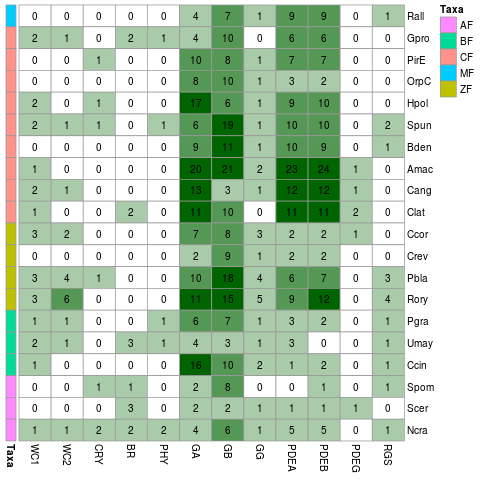
\includegraphics[]{./Chapter_RhodAux/img/photosenseHeatmap.png}
  \caption[Photosensory survey]{Photosensory protein distribution and G protein signaling pathway component distribution. Protein abbreviations: WC1, WC2=White collar 1 and 2; CRY=Cryptochrome; PHY=Phytochrome; BR=Bacterialrhodopsin (Type 1); GA, GB, GG=G protein subunits G$\alpha$, G$\beta$, and G$\gamma$; PDEA, PDEB, and PDEG=Phosphodiesterase subunits PDE$\alpha$, PDE$\beta$, and PDE$\gamma$; RGS=Regulator of G protein signaling. For species abbreviations, refer to Table~\ref{tab:AppData_taxa}}
  \label{fig:ChRhodA_photosenseSurvey}
\end{figure}

% Galpha msa
\begin{figure}[hb]
  \centering
  \begin{texshade}{./Chapter_RhodAux/dat/FungalGA_PM.fasta_aln}
    \threshold[80]{50}
    \setdomain{1}{1..15,340..355}
    \showruler{1}{top}
    \feature{top}{1}{MGXXXS}{brace[Red]}{Myristoylation [Red]}
    \feature{top}{1}{351..355}{brace[Blue]}{Pertussis [Blue]}
    \hidenumbering
  \end{texshade}
  \caption[G$\alpha$ MSA]{Multiple sequence aligment of N-termini and C-termini. G$\alpha$ proteins identified in fungi which posessed both N-terminal myristoylation (MGXXXS) and C-terminal pertussis (C[GAVLIP]\{2\}X) motifs were aligned using T-coffee.}
  \label{fig:ChRhodA_gaMSA}
\end{figure}

% Galpha tree, group1
\begin{figure}[hb]
  \centering
  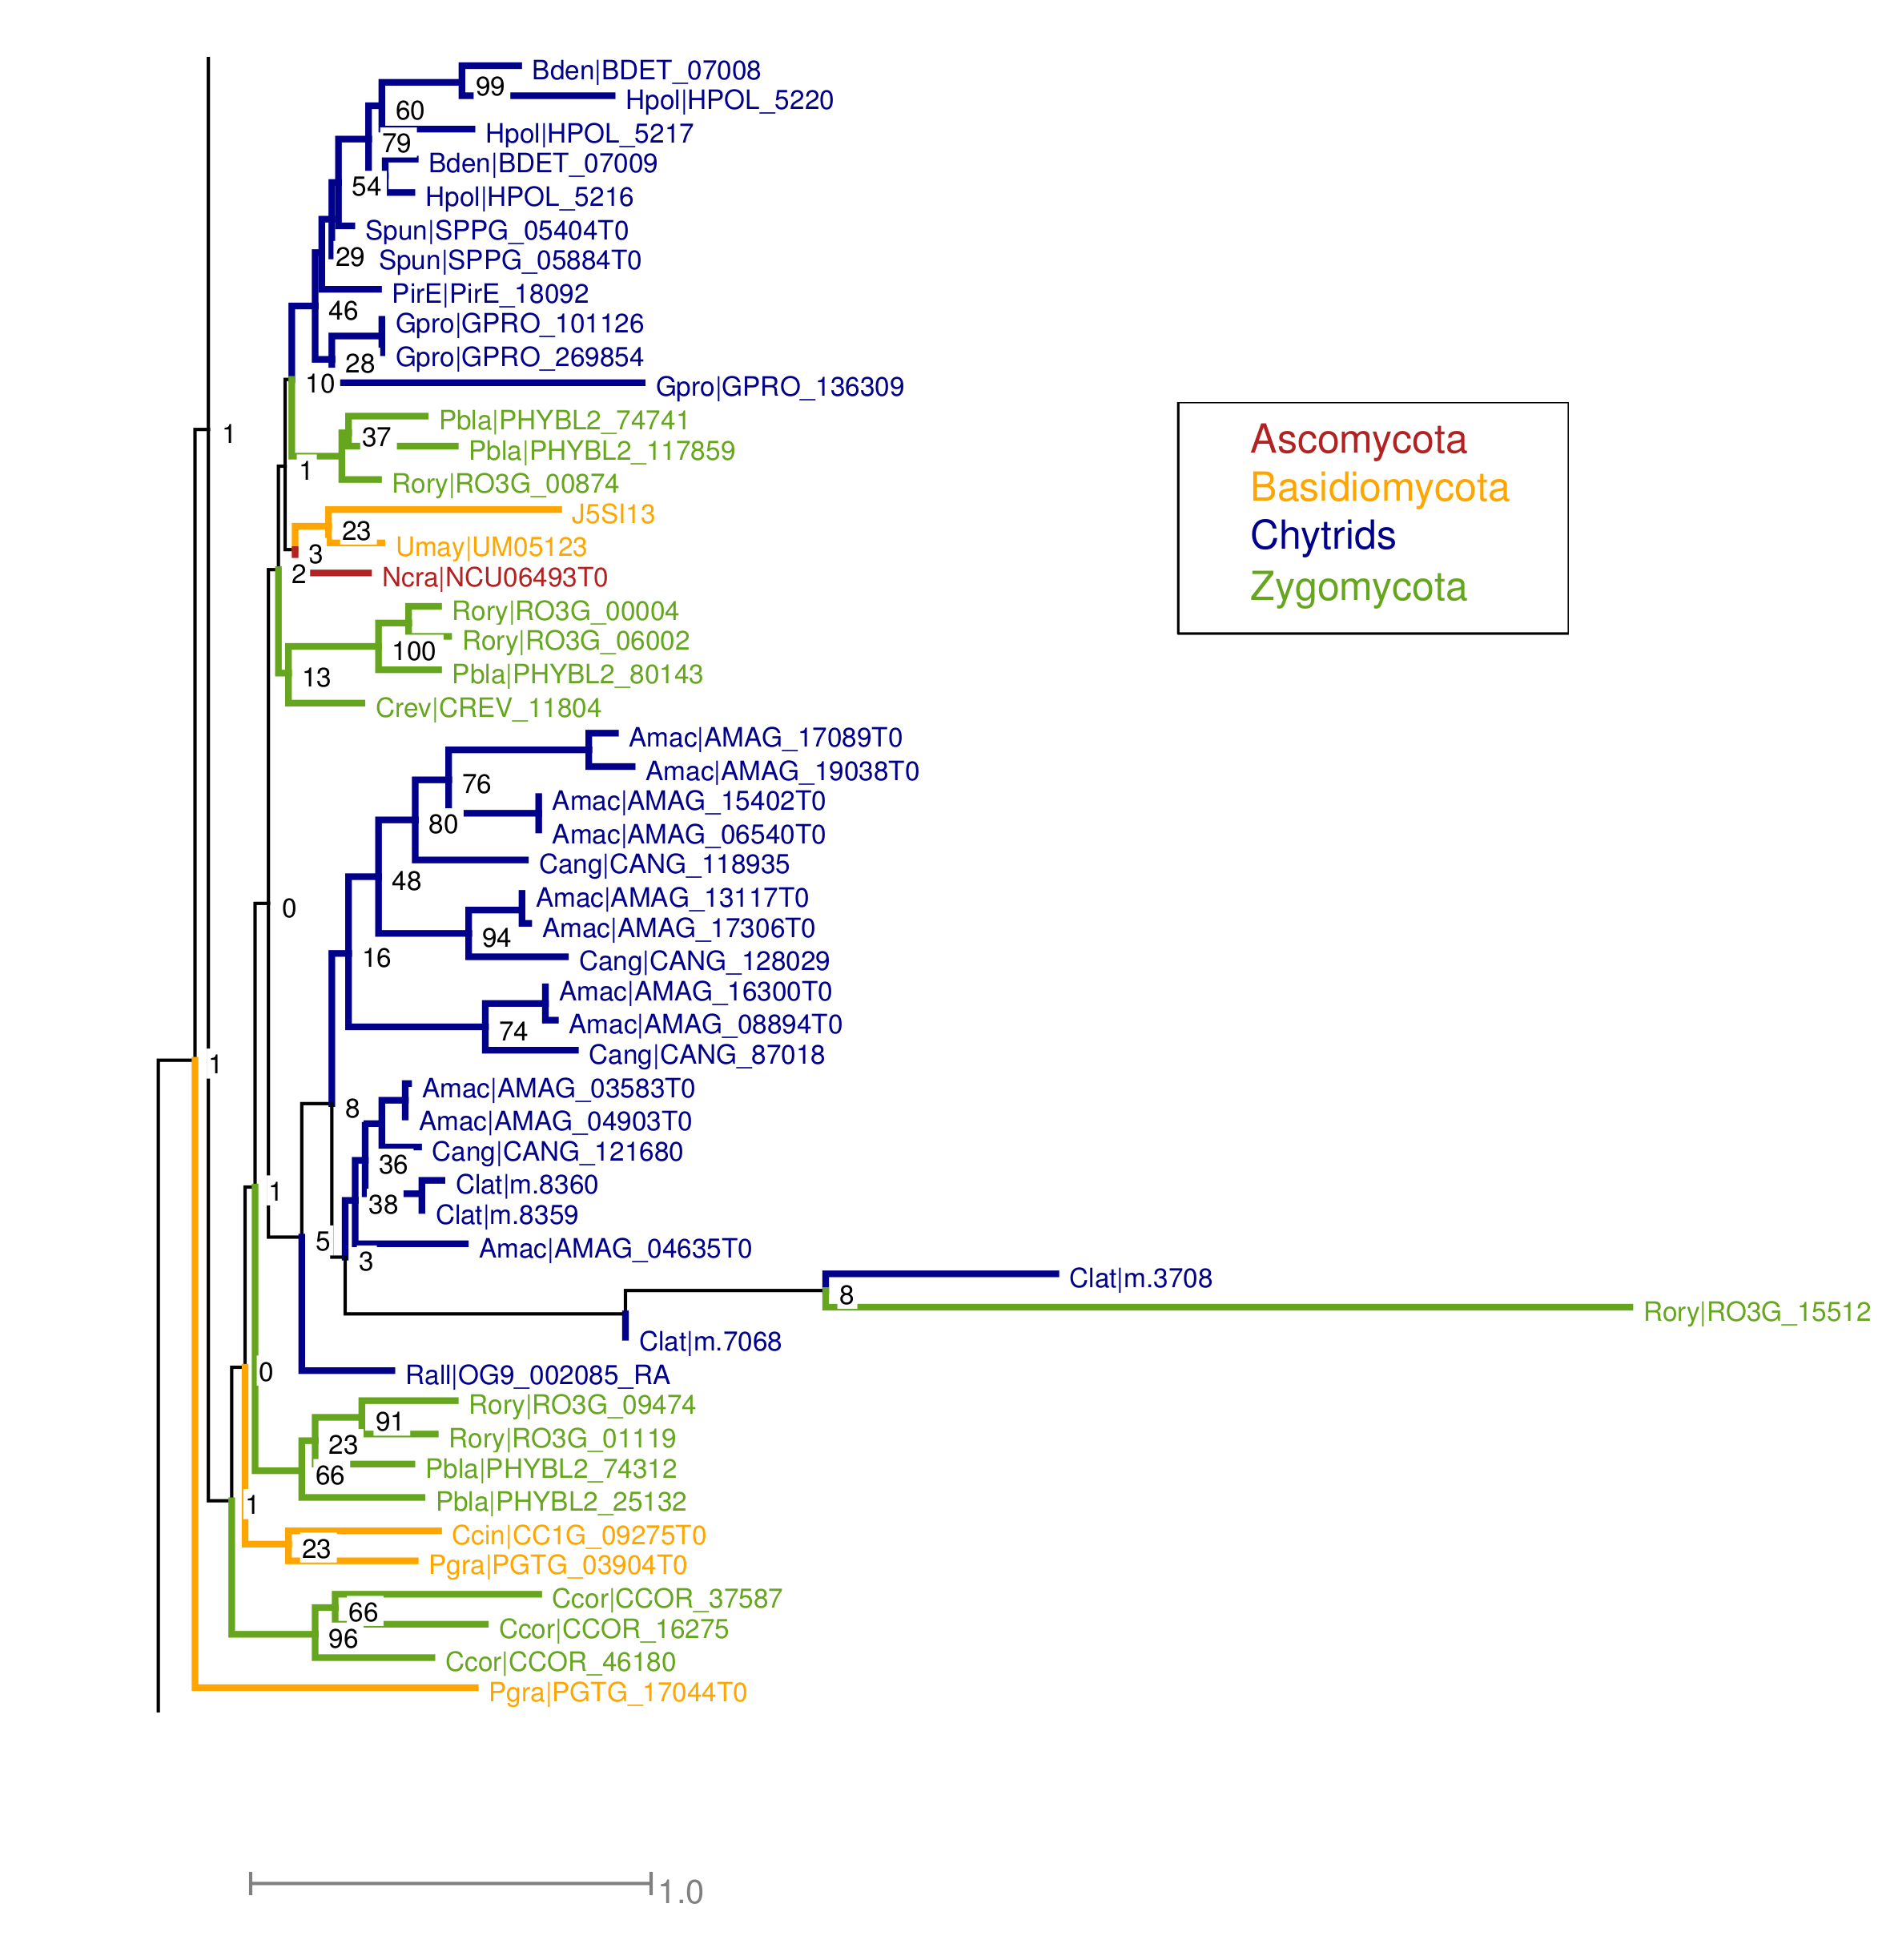
\includegraphics{./Chapter_RhodAux/img/Galpha_tree_grp1.png}
  \caption[G$\alpha$ tree, group 1]{Maximum likelihood tree of identified G-$\alpha$ subunits in fungi (group I, as defined by inclusion of NCU06493)}
  \label{fig:ChRhodA_GalphaTree1}
\end{figure}

% Galpha tree, group2
\begin{figure}[hb]
  \centering
  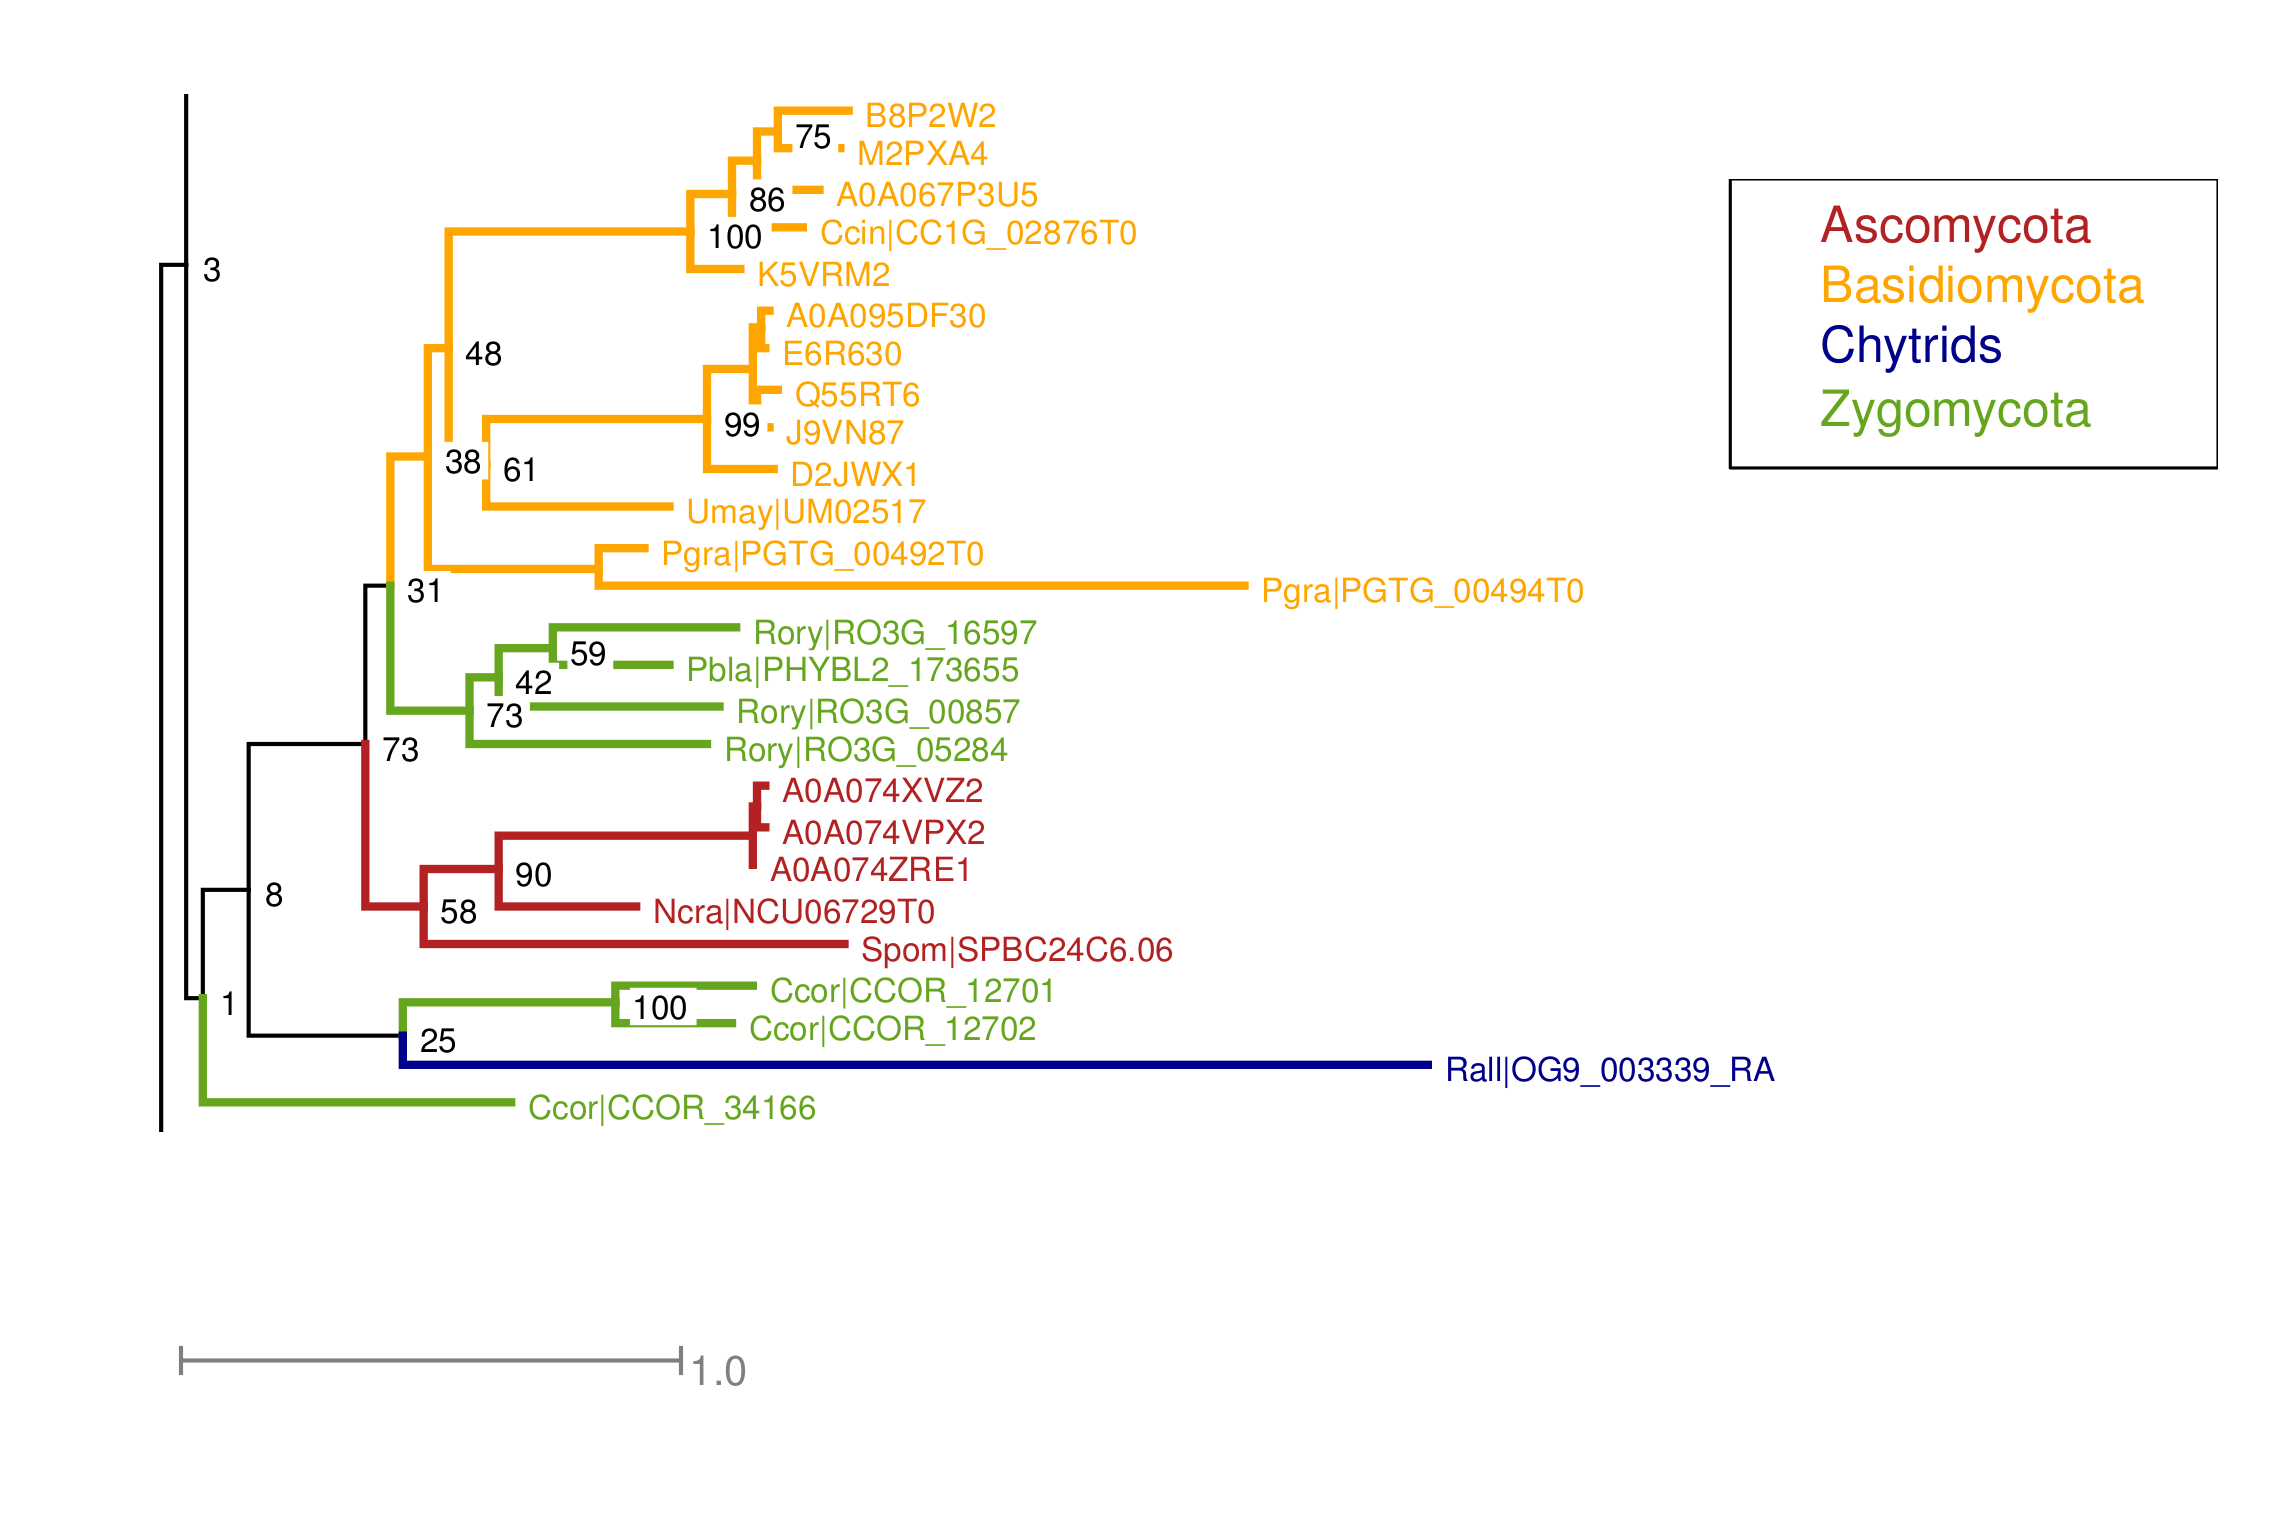
\includegraphics{./Chapter_RhodAux/img/Galpha_tree_grp2.png}
  \caption[G$\alpha$ tree, group2]{Maximum likelihood tree of identified G-$\alpha$ subunits in fungi (group II, as defined by inclusion of NCU06729)}
  \label{fig:ChRhodA_GalphaTree2}
\end{figure}

% Galpha tree, group3
\begin{figure}[hb]
  \centering
  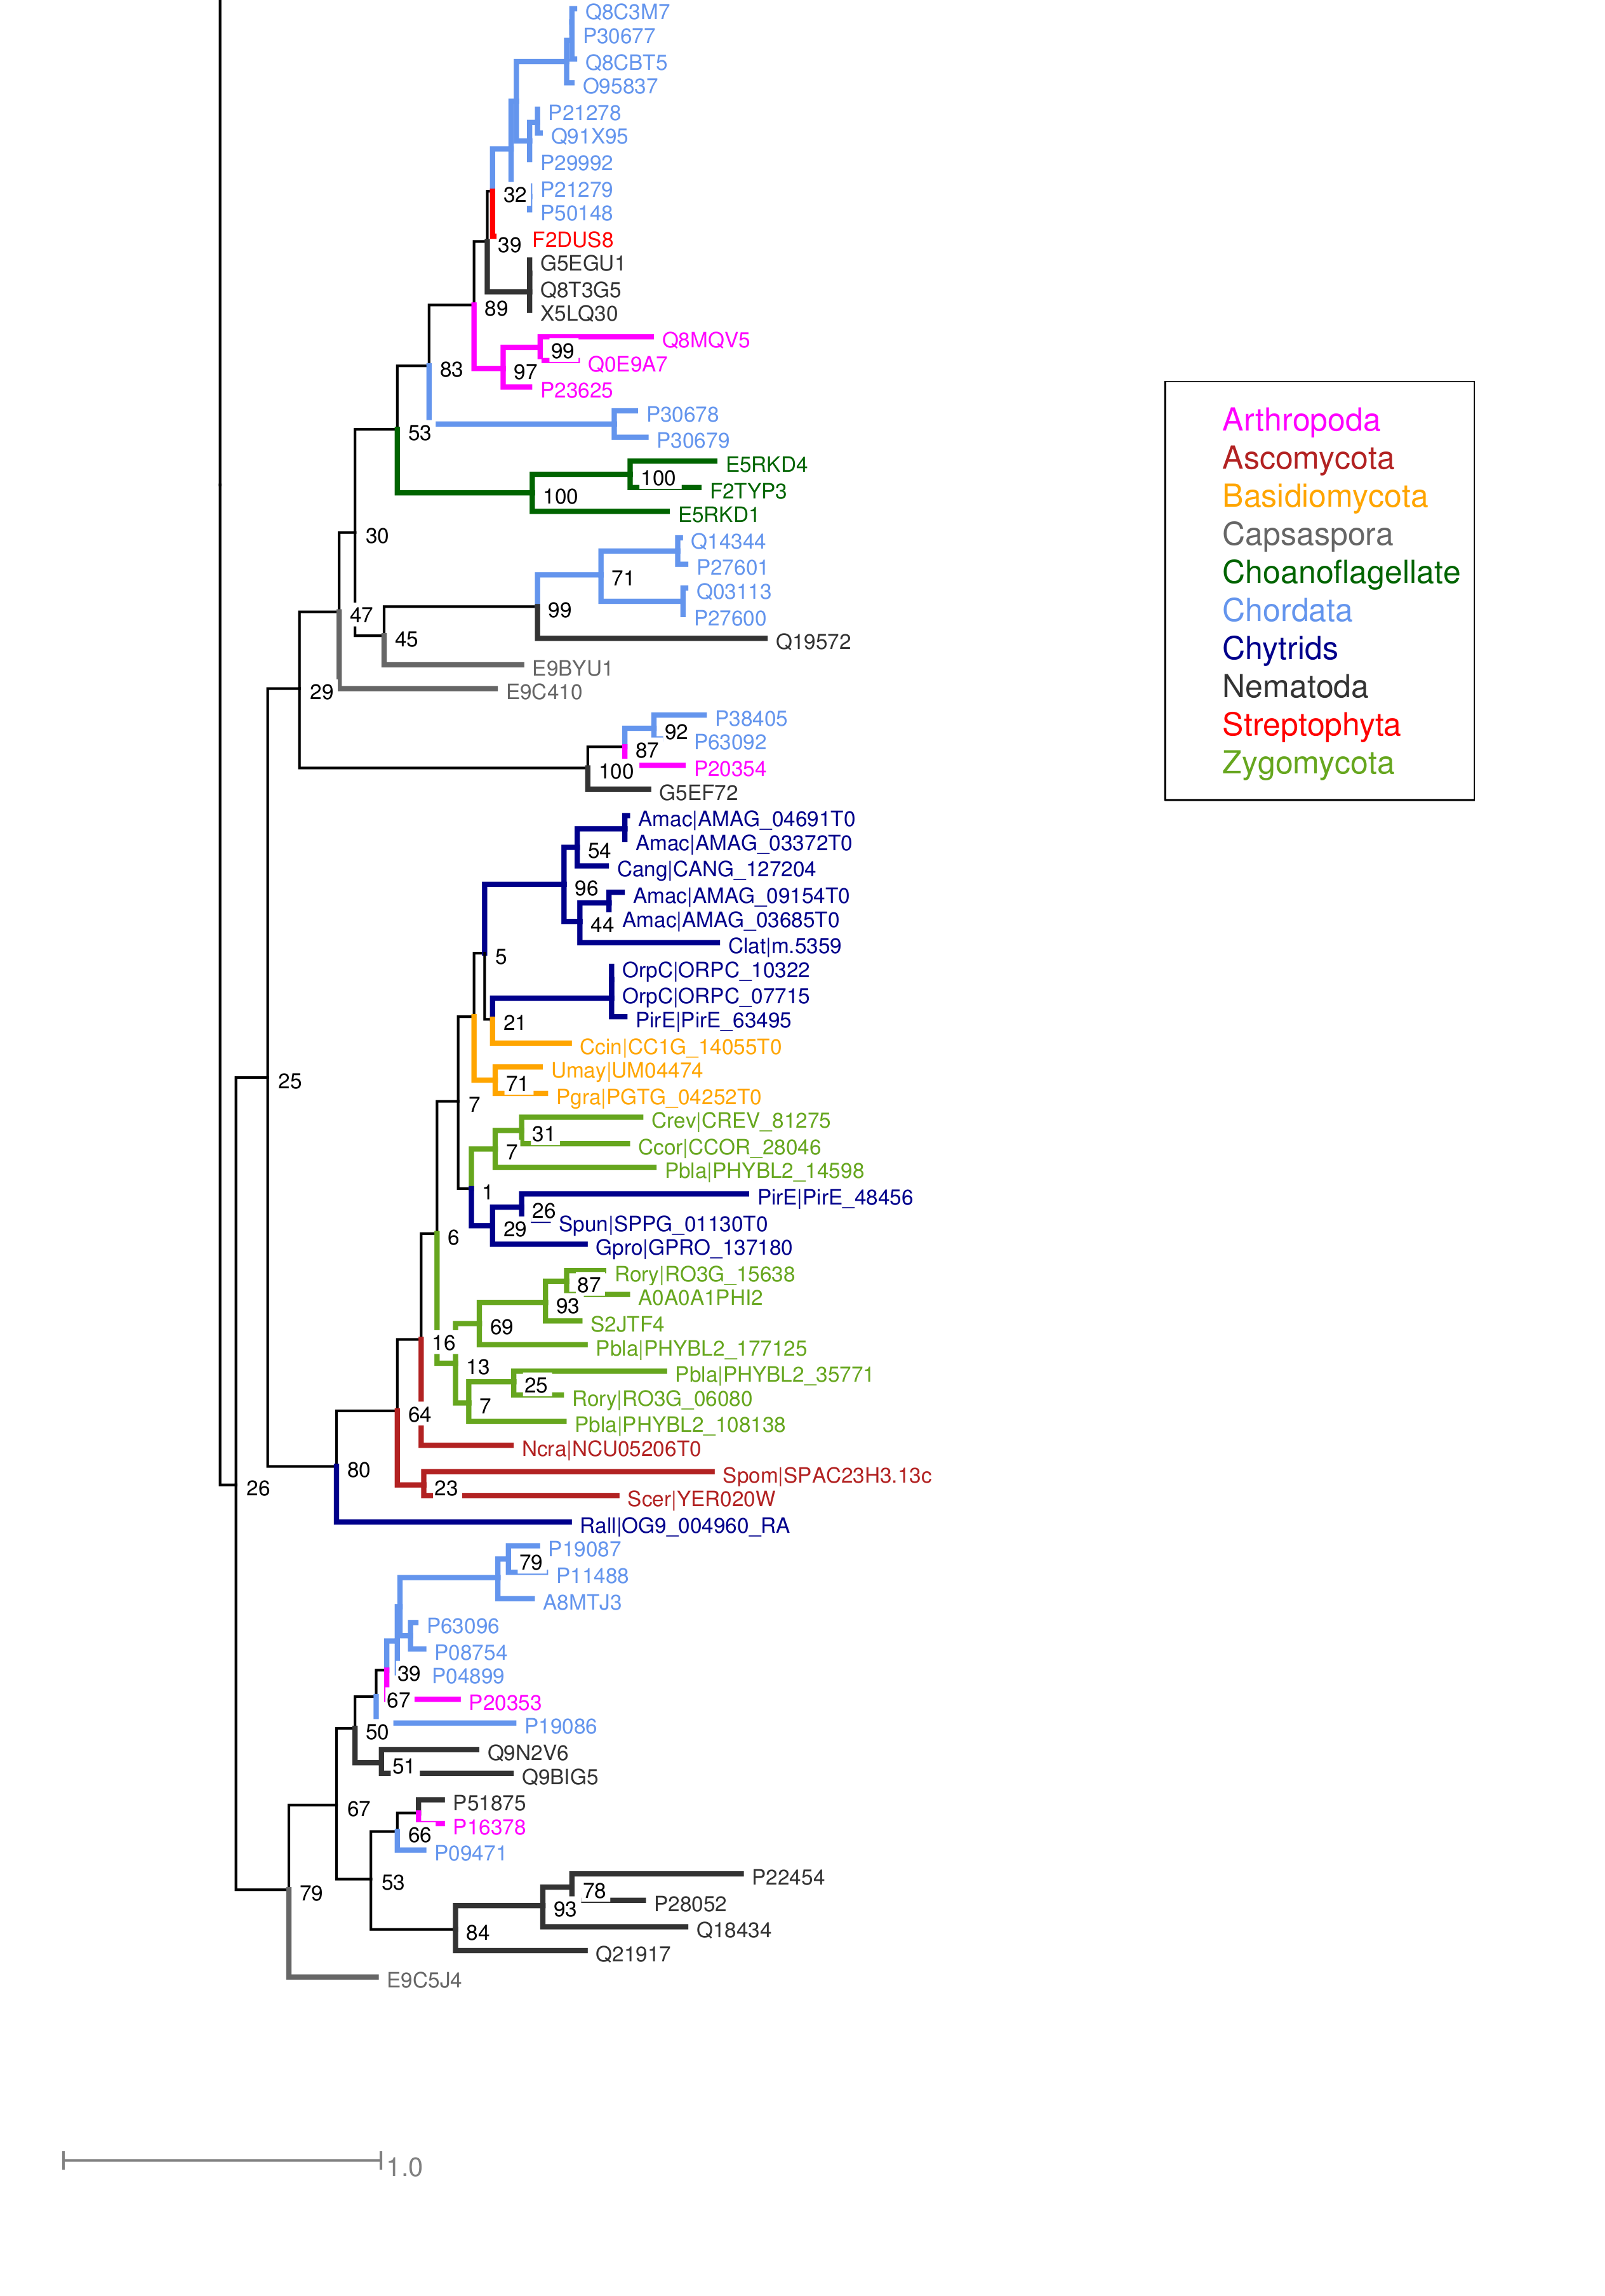
\includegraphics{./Chapter_RhodAux/img/Galpha_tree_grp3_outGroups.png}
  \caption[G$\alpha$ tree, group3]{Maximum likelihood tree of identified G-$\alpha$ subunits in fungi (group III, as defined by inclusion of NCU05206) and outgroups}
  \label{fig:ChRhodA_GalphaTree3}
\end{figure}

% Galpha tree, group4
\begin{figure}[hb]
  \centering
  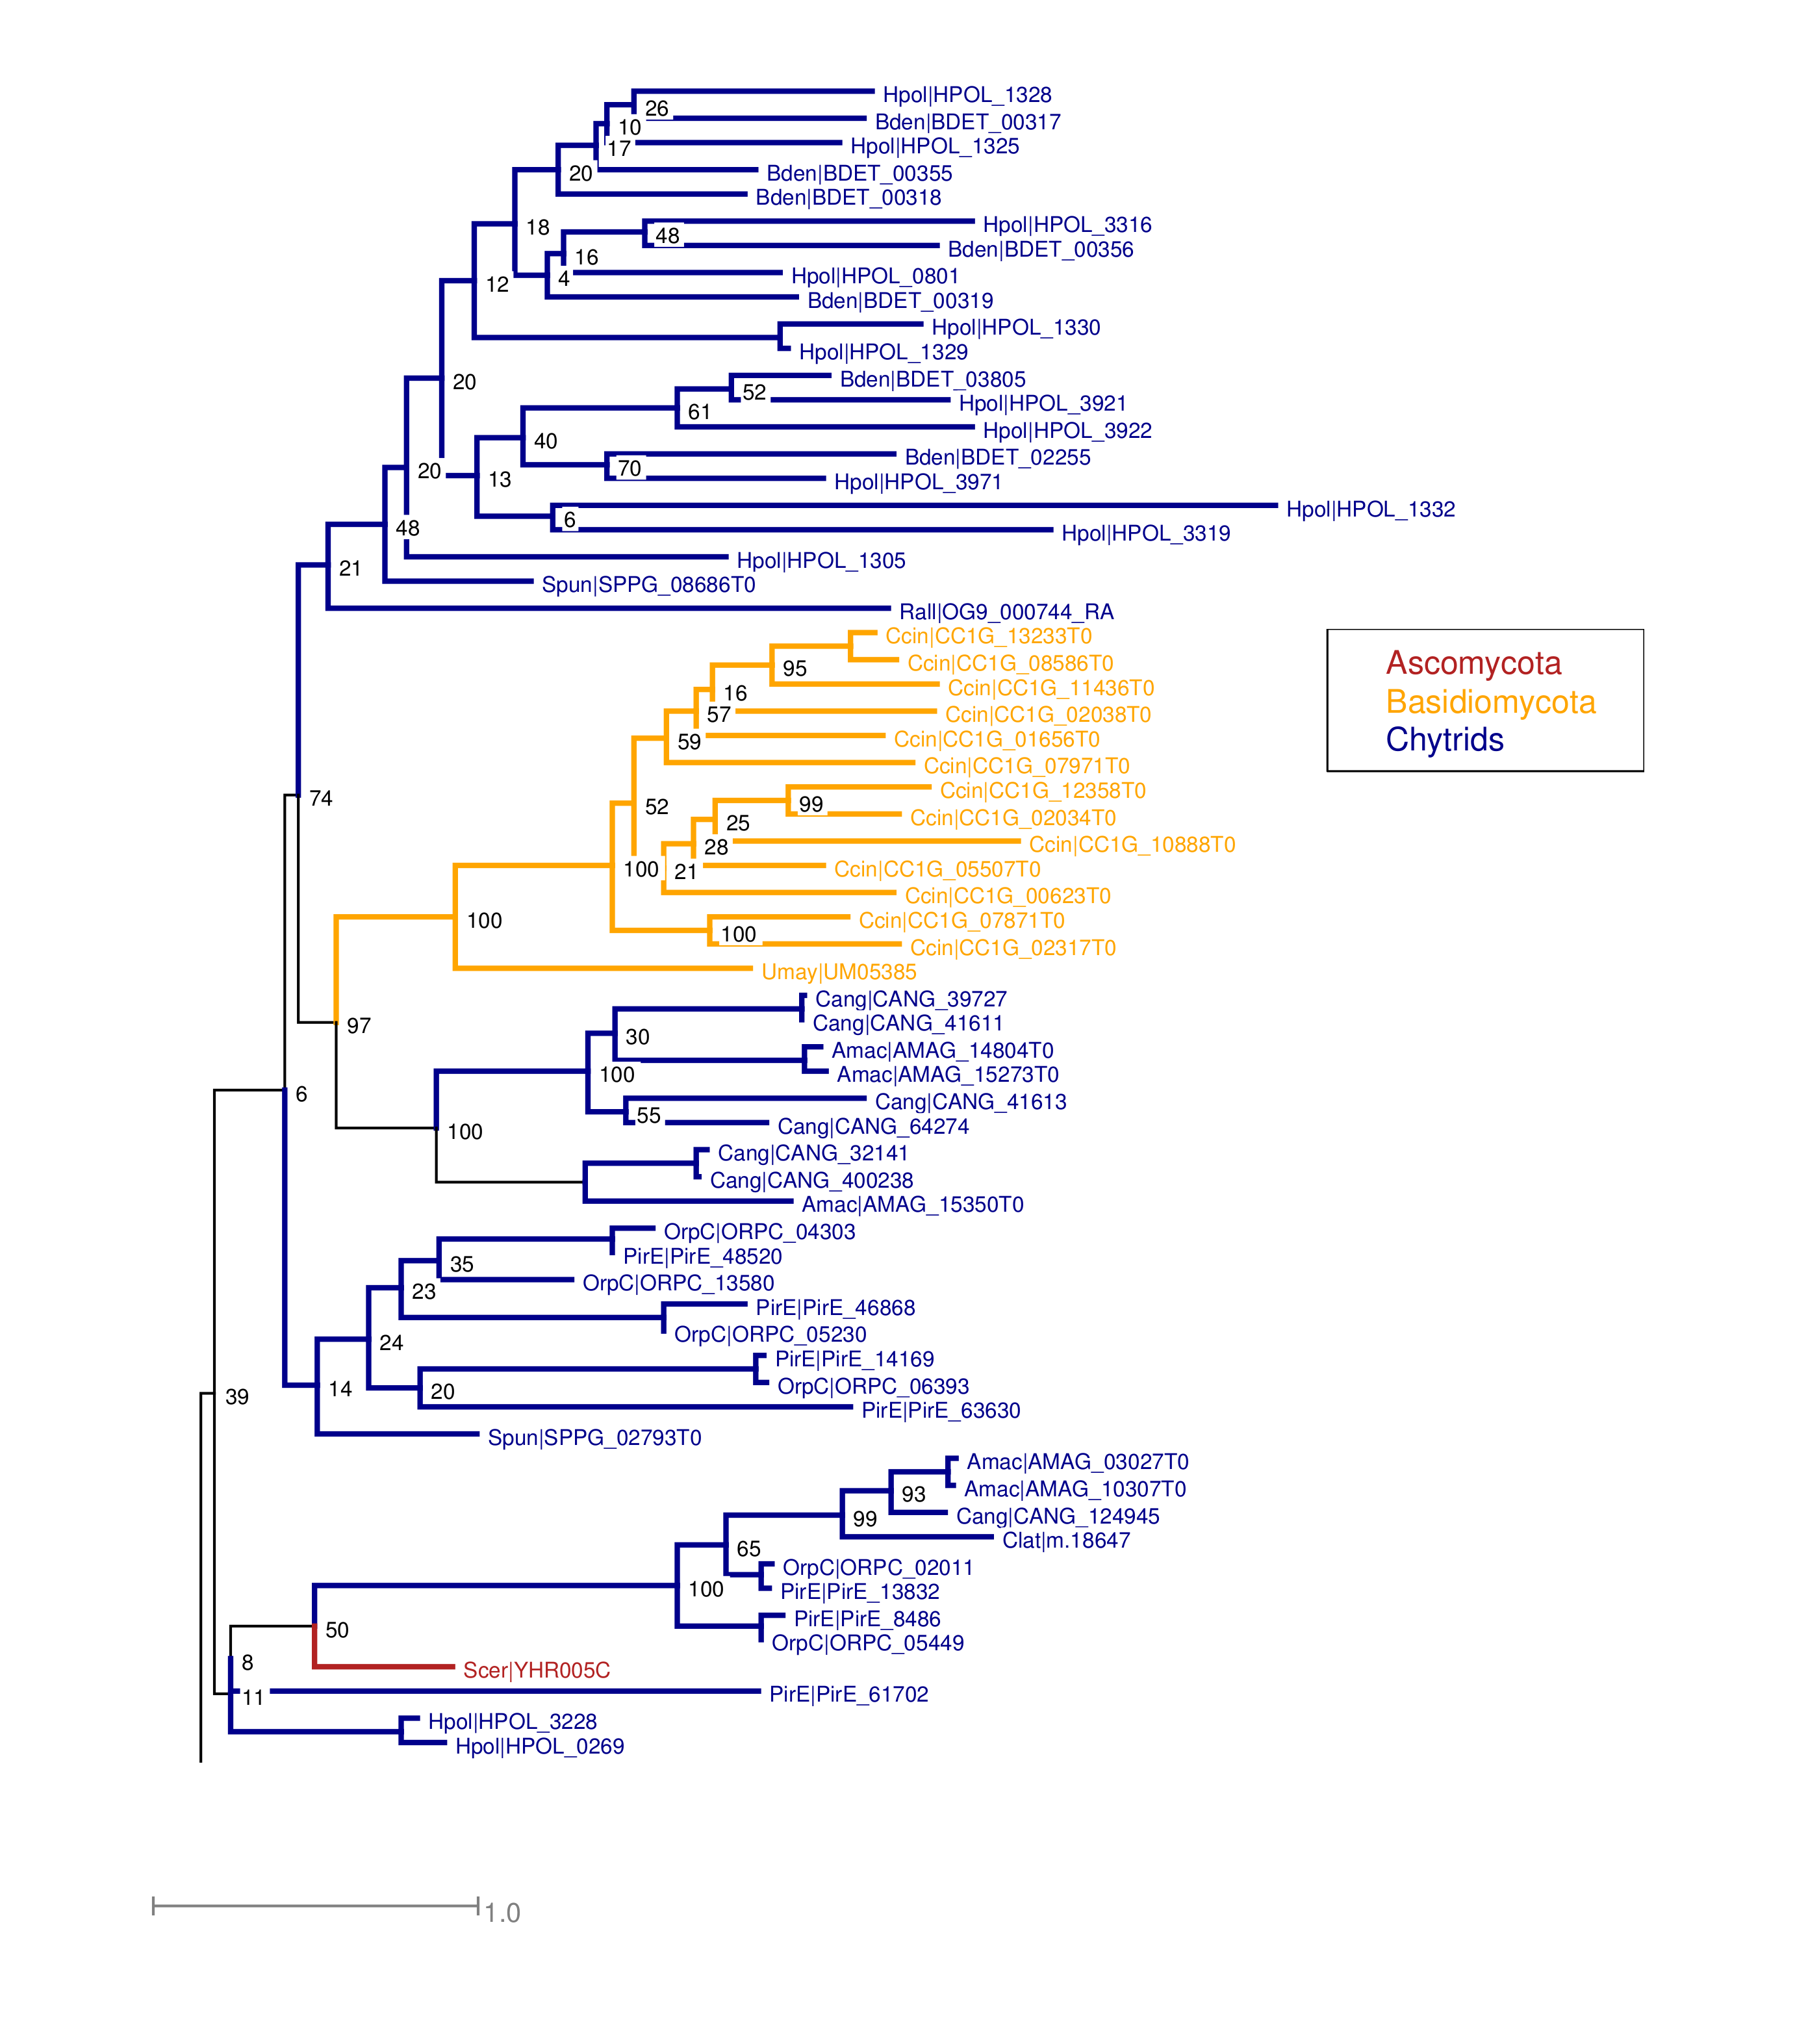
\includegraphics{./Chapter_RhodAux/img/Galpha_tree_grp4.png}
  \caption[G$\alpha$ tree, group4]{Maximum likelihood tree of identified G-$\alpha$ subunits in fungi (group IV, as defined by absence of \textit{N. crassa} homologs and inclusion of UM05385 from \textit{Ustilago maydis})}
  \label{fig:ChRhodA_GalphaTree4}
\end{figure}

% Gbeta structure
\begin{figure}[hb]
  \centering
  \begin{texshade}{./Chapter_RhodAux/dat/FungalGB.fasta_aln}
    \shadingmode[allmatchspecial]{similar}
    \shadingcolors{grays}
    \fingerprint{500}
    \showlegend
    \feature{top}{NCU00440T0}{61..98,153..186,233..271,111..140,289..315,191..229,321..356}{,-,}{WD}
  \end{texshade}
  \caption[G$\beta$ WD40 repeats]{Schematic of identified fungal G$\beta$ proteins highlighting conservation and location of multiple WD40 repeat domains}
  \label{fig:ChRhodA_GbetaStruct}
\end{figure}

% Gbeta tree
\begin{figure}[hb]
  \centering
  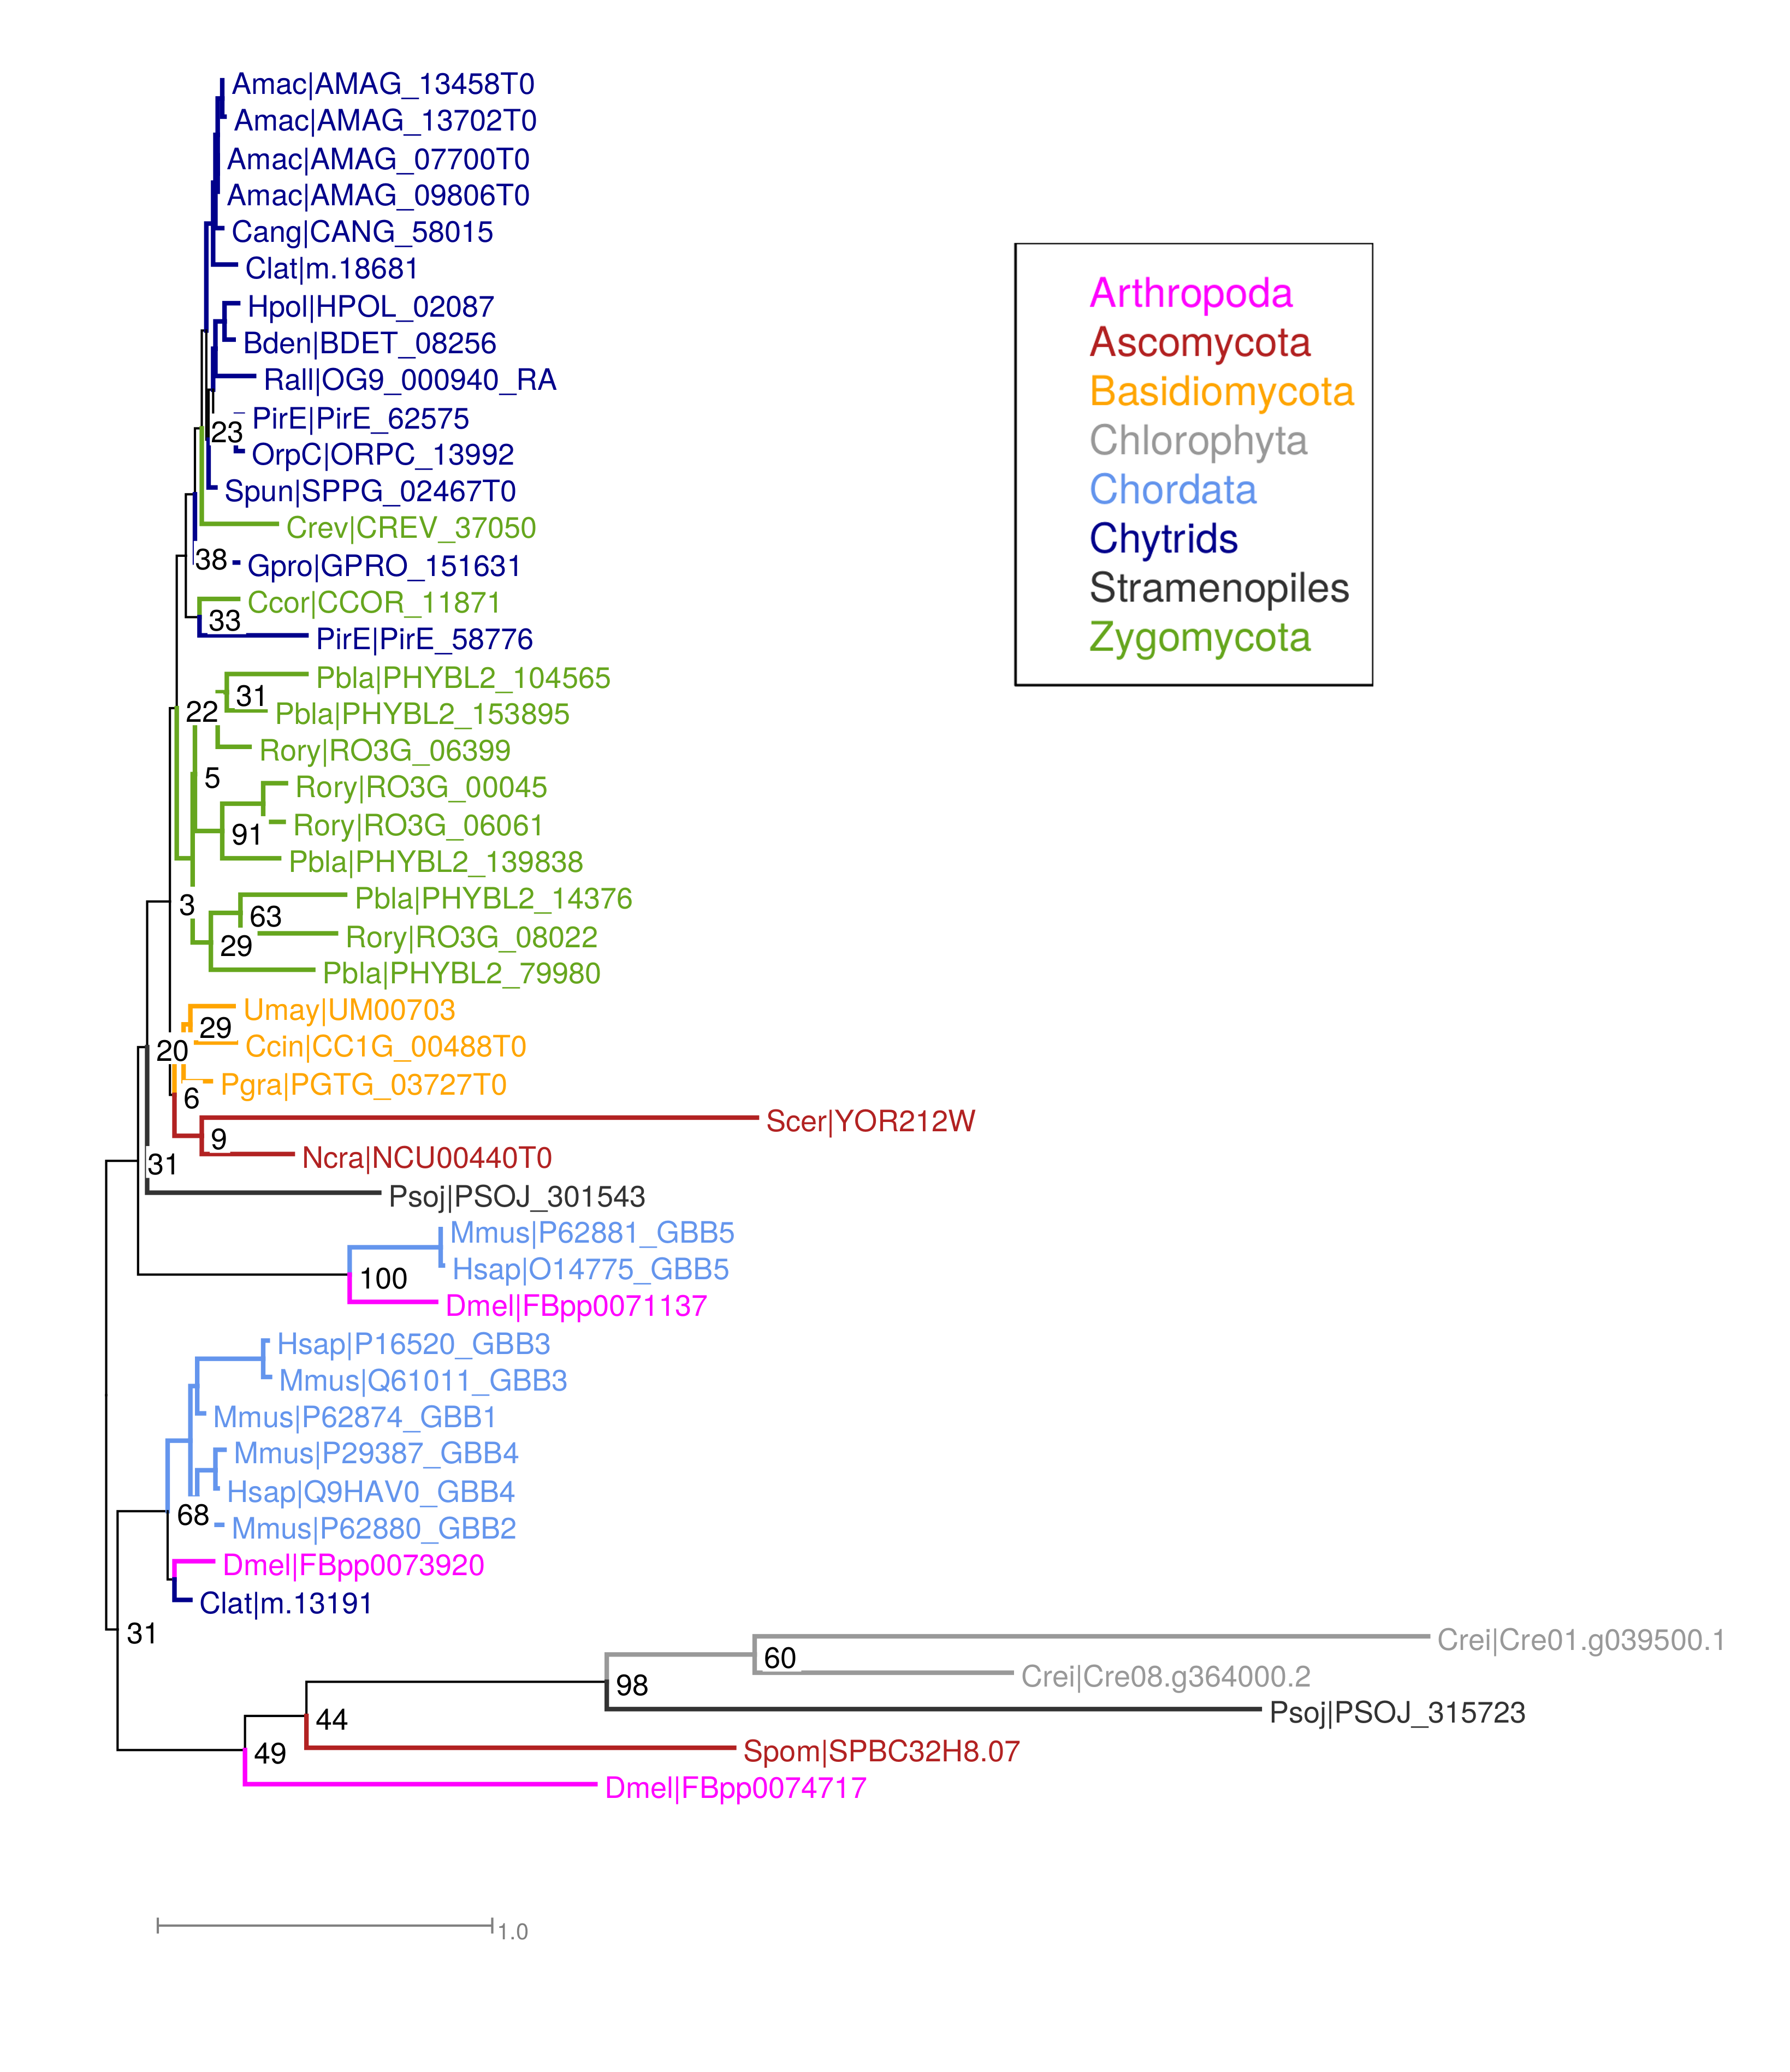
\includegraphics{./Chapter_RhodAux/img/Gbeta_tree.png}
  \caption[G$\beta$ tree]{Maximum likelihood tree of identified G$\beta$ subunits in fungi and animal outgroups}
  \label{fig:ChRhodA_GbetaTree}
\end{figure}

% Ggamma msa
\begin{figure}[hb]
  \centering
  \begin{texshade}{./Chapter_RhodAux/dat/FungalGG.fasta_aln}
    \threshold[80]{50}
    \setends{1}{45..70}
    \showruler{1}{top}
    \feature{top}{1}{62..65}{brace[Blue]}{Pertussis [Blue]}
    \hidenumbering
  \end{texshade}
  \caption[G$\gamma$ MSA]{Multiple sequence aligment of C-termini of G$\gamma$ proteins identified in fungi which posessed C-terminal pertussis (C[GAVLIP]\{2\}X) motifs aligned using T-coffee.}
  \label{fig:ChRhodA_ggMSA}
\end{figure}

% Ggamma tree
\begin{figure}[hb]
  \centering
  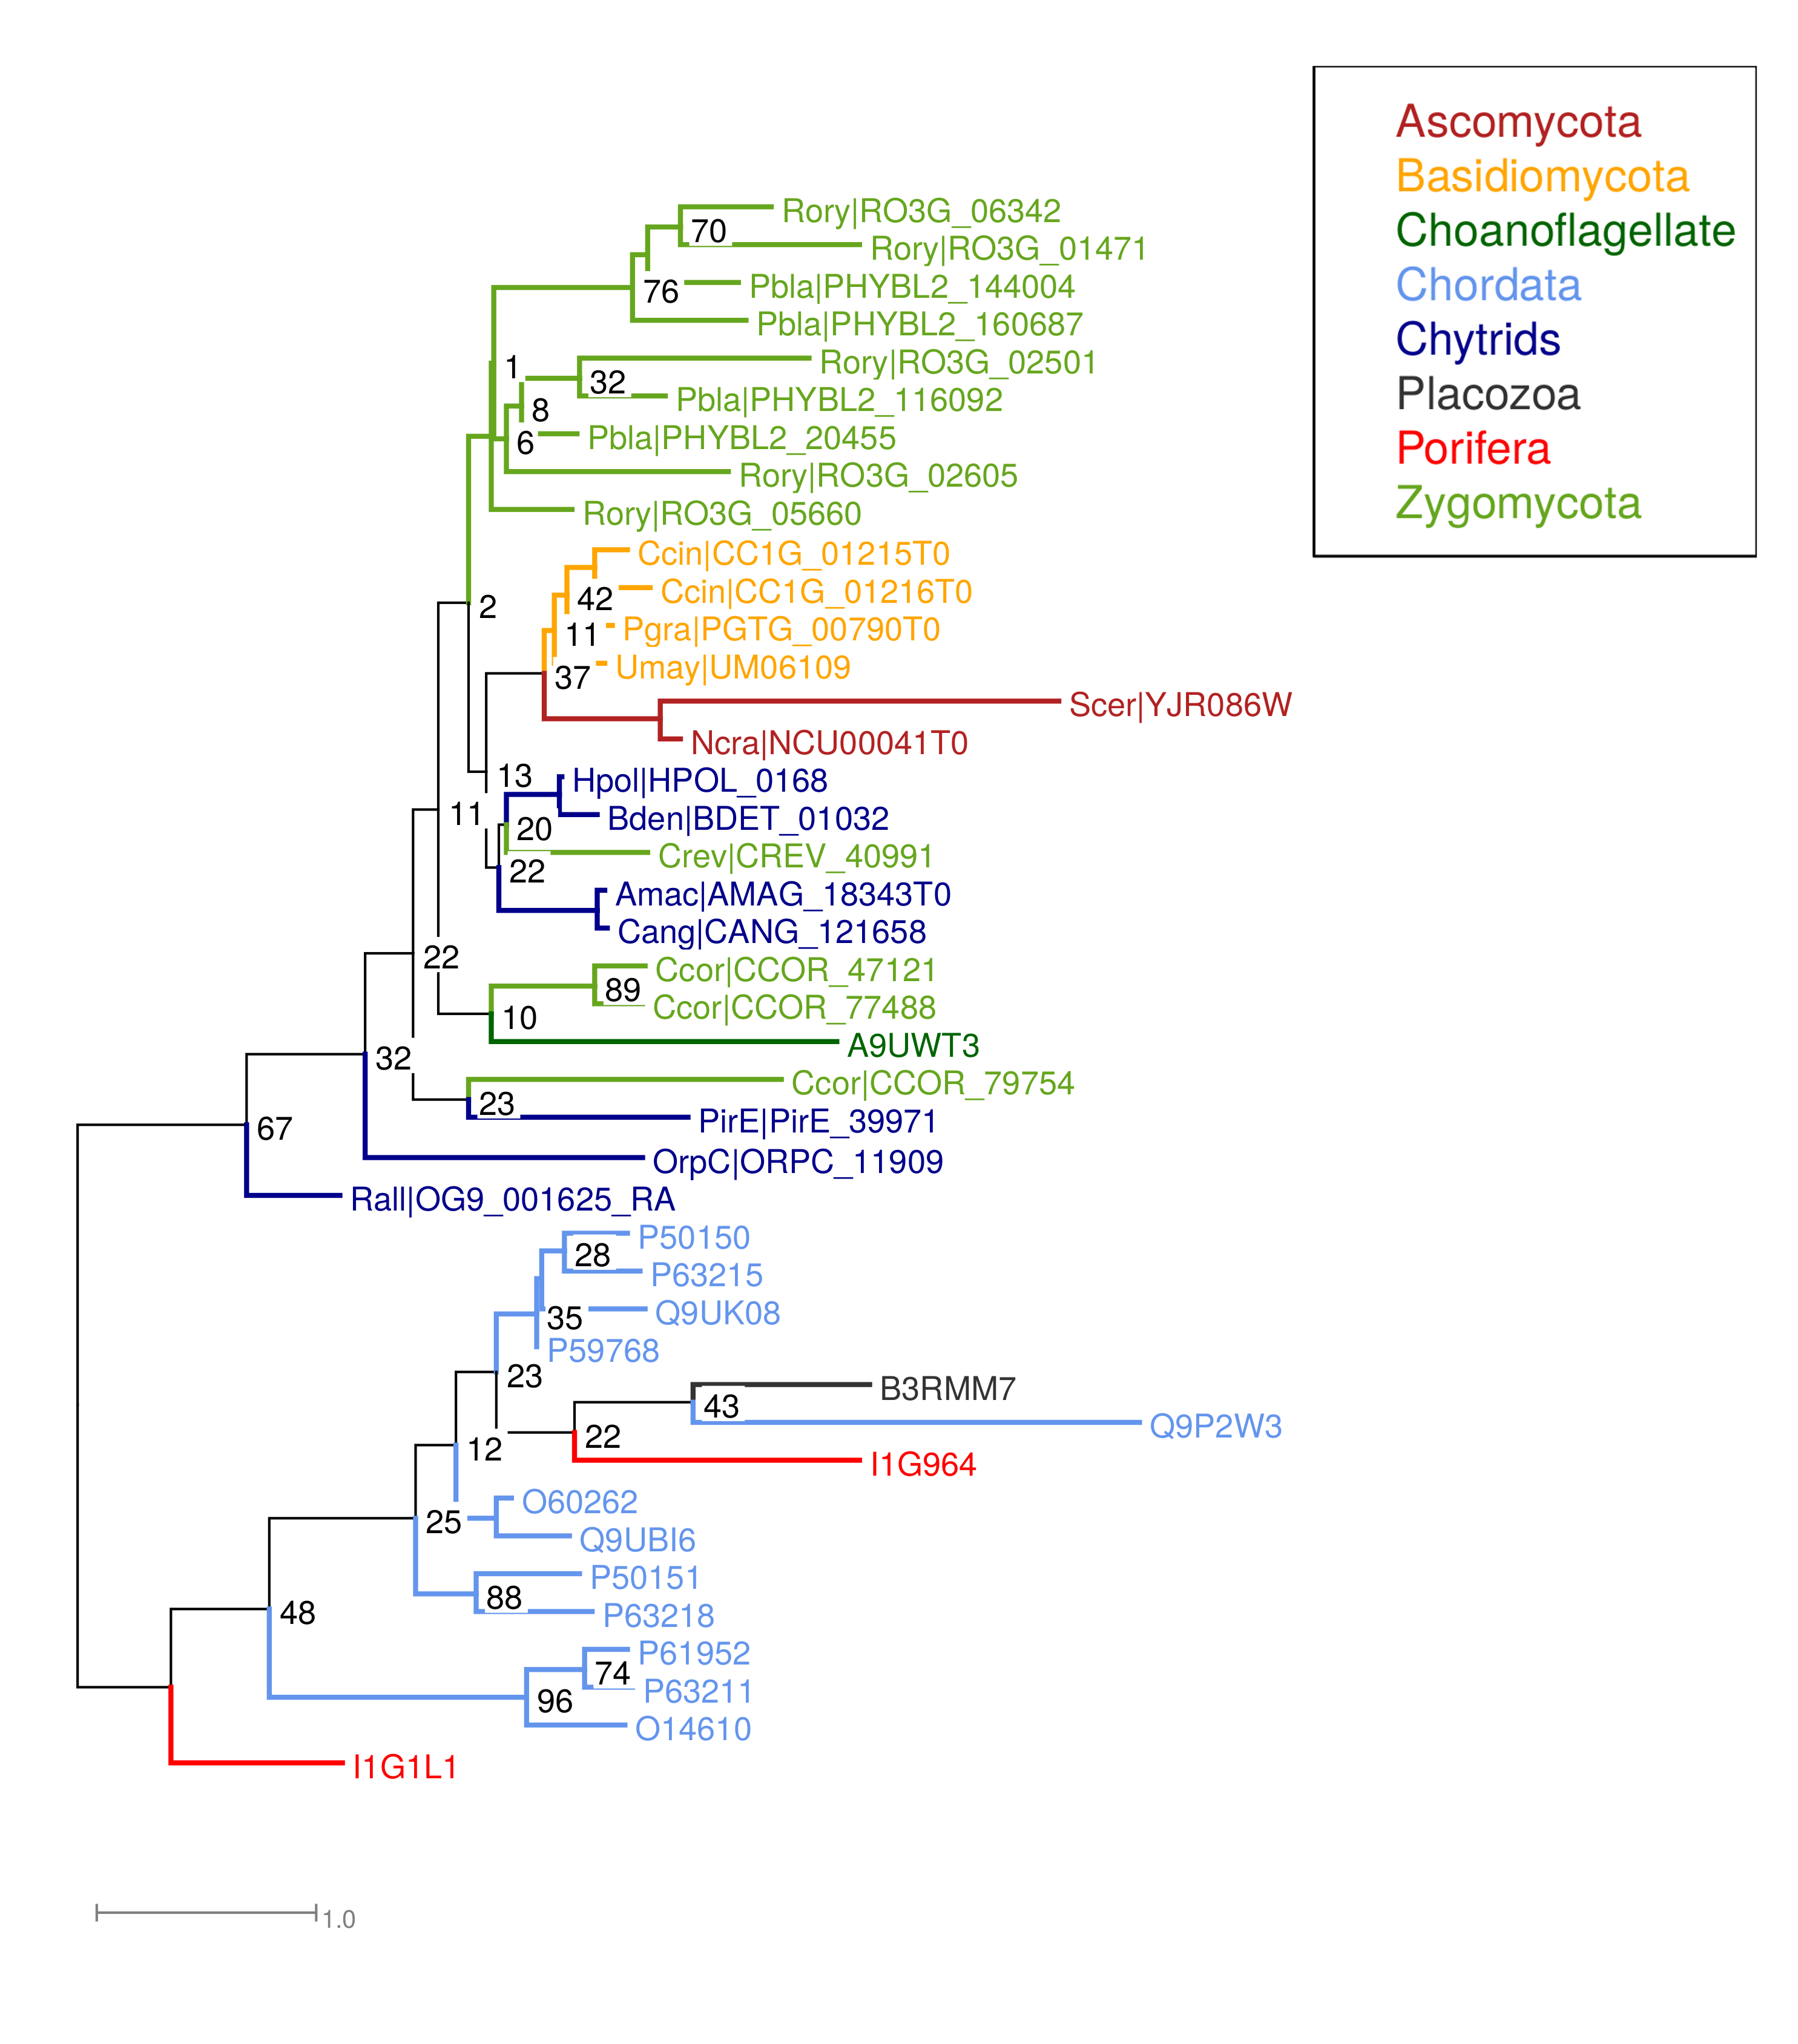
\includegraphics{./Chapter_RhodAux/img/Ggamma_tree.png}
  \caption[G$\gamma$ tree]{Maximum likelihood tree of identified G$\gamma$ subunits in fungi and animal outgroups}
  \label{fig:ChRhodA_GgammaTree}
\end{figure}

% RGS structure
\begin{figure}[hb]
  \centering
  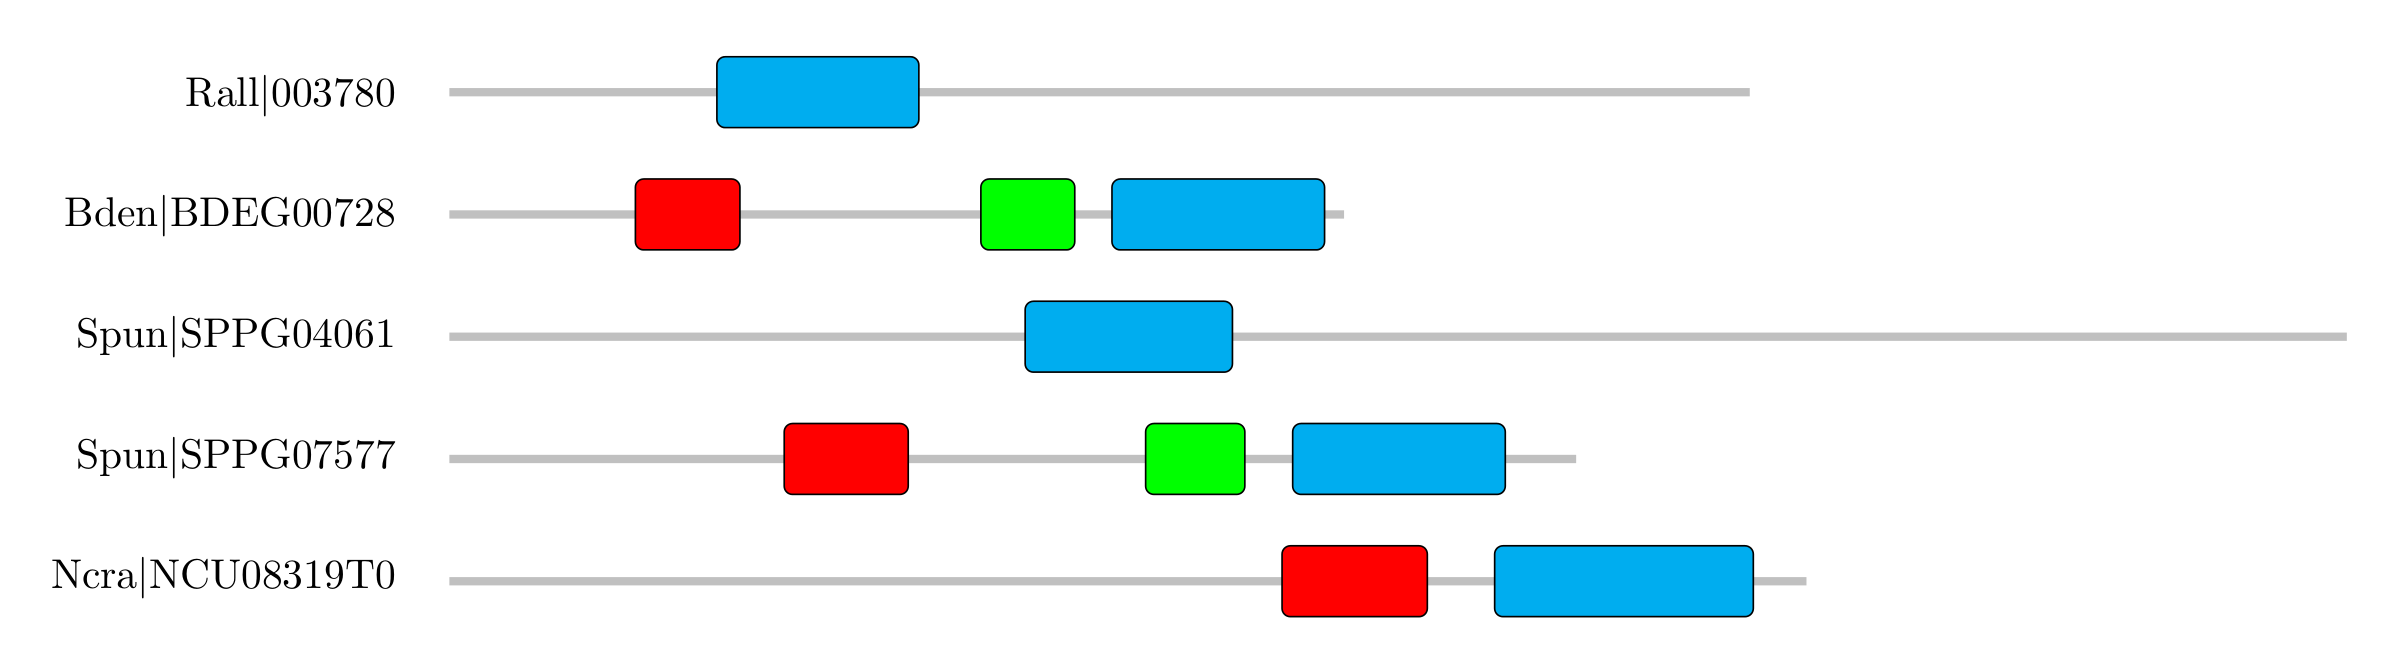
\includegraphics{./Chapter_RhodAux/img/ChyNcra_RGS.png}
  \caption[RGS proteins]{Structural domains of RGS proteins identified from HMM search in chytrids. Fungal hits contain RGS-domains (PF00615; blue). The \textit{Bd} hit and one \textit{Sp} hit additionally contain GGL (PF00631; green) and DEP (PF00610; red) domains. A second \textit{Sp} hit, and the hit from \textit{Rozella} only contain the RGS domain.}
  \label{fig:ChRhodA_RGS}
\end{figure}

% PDE tree
\begin{figure}[hb]
  \centering
  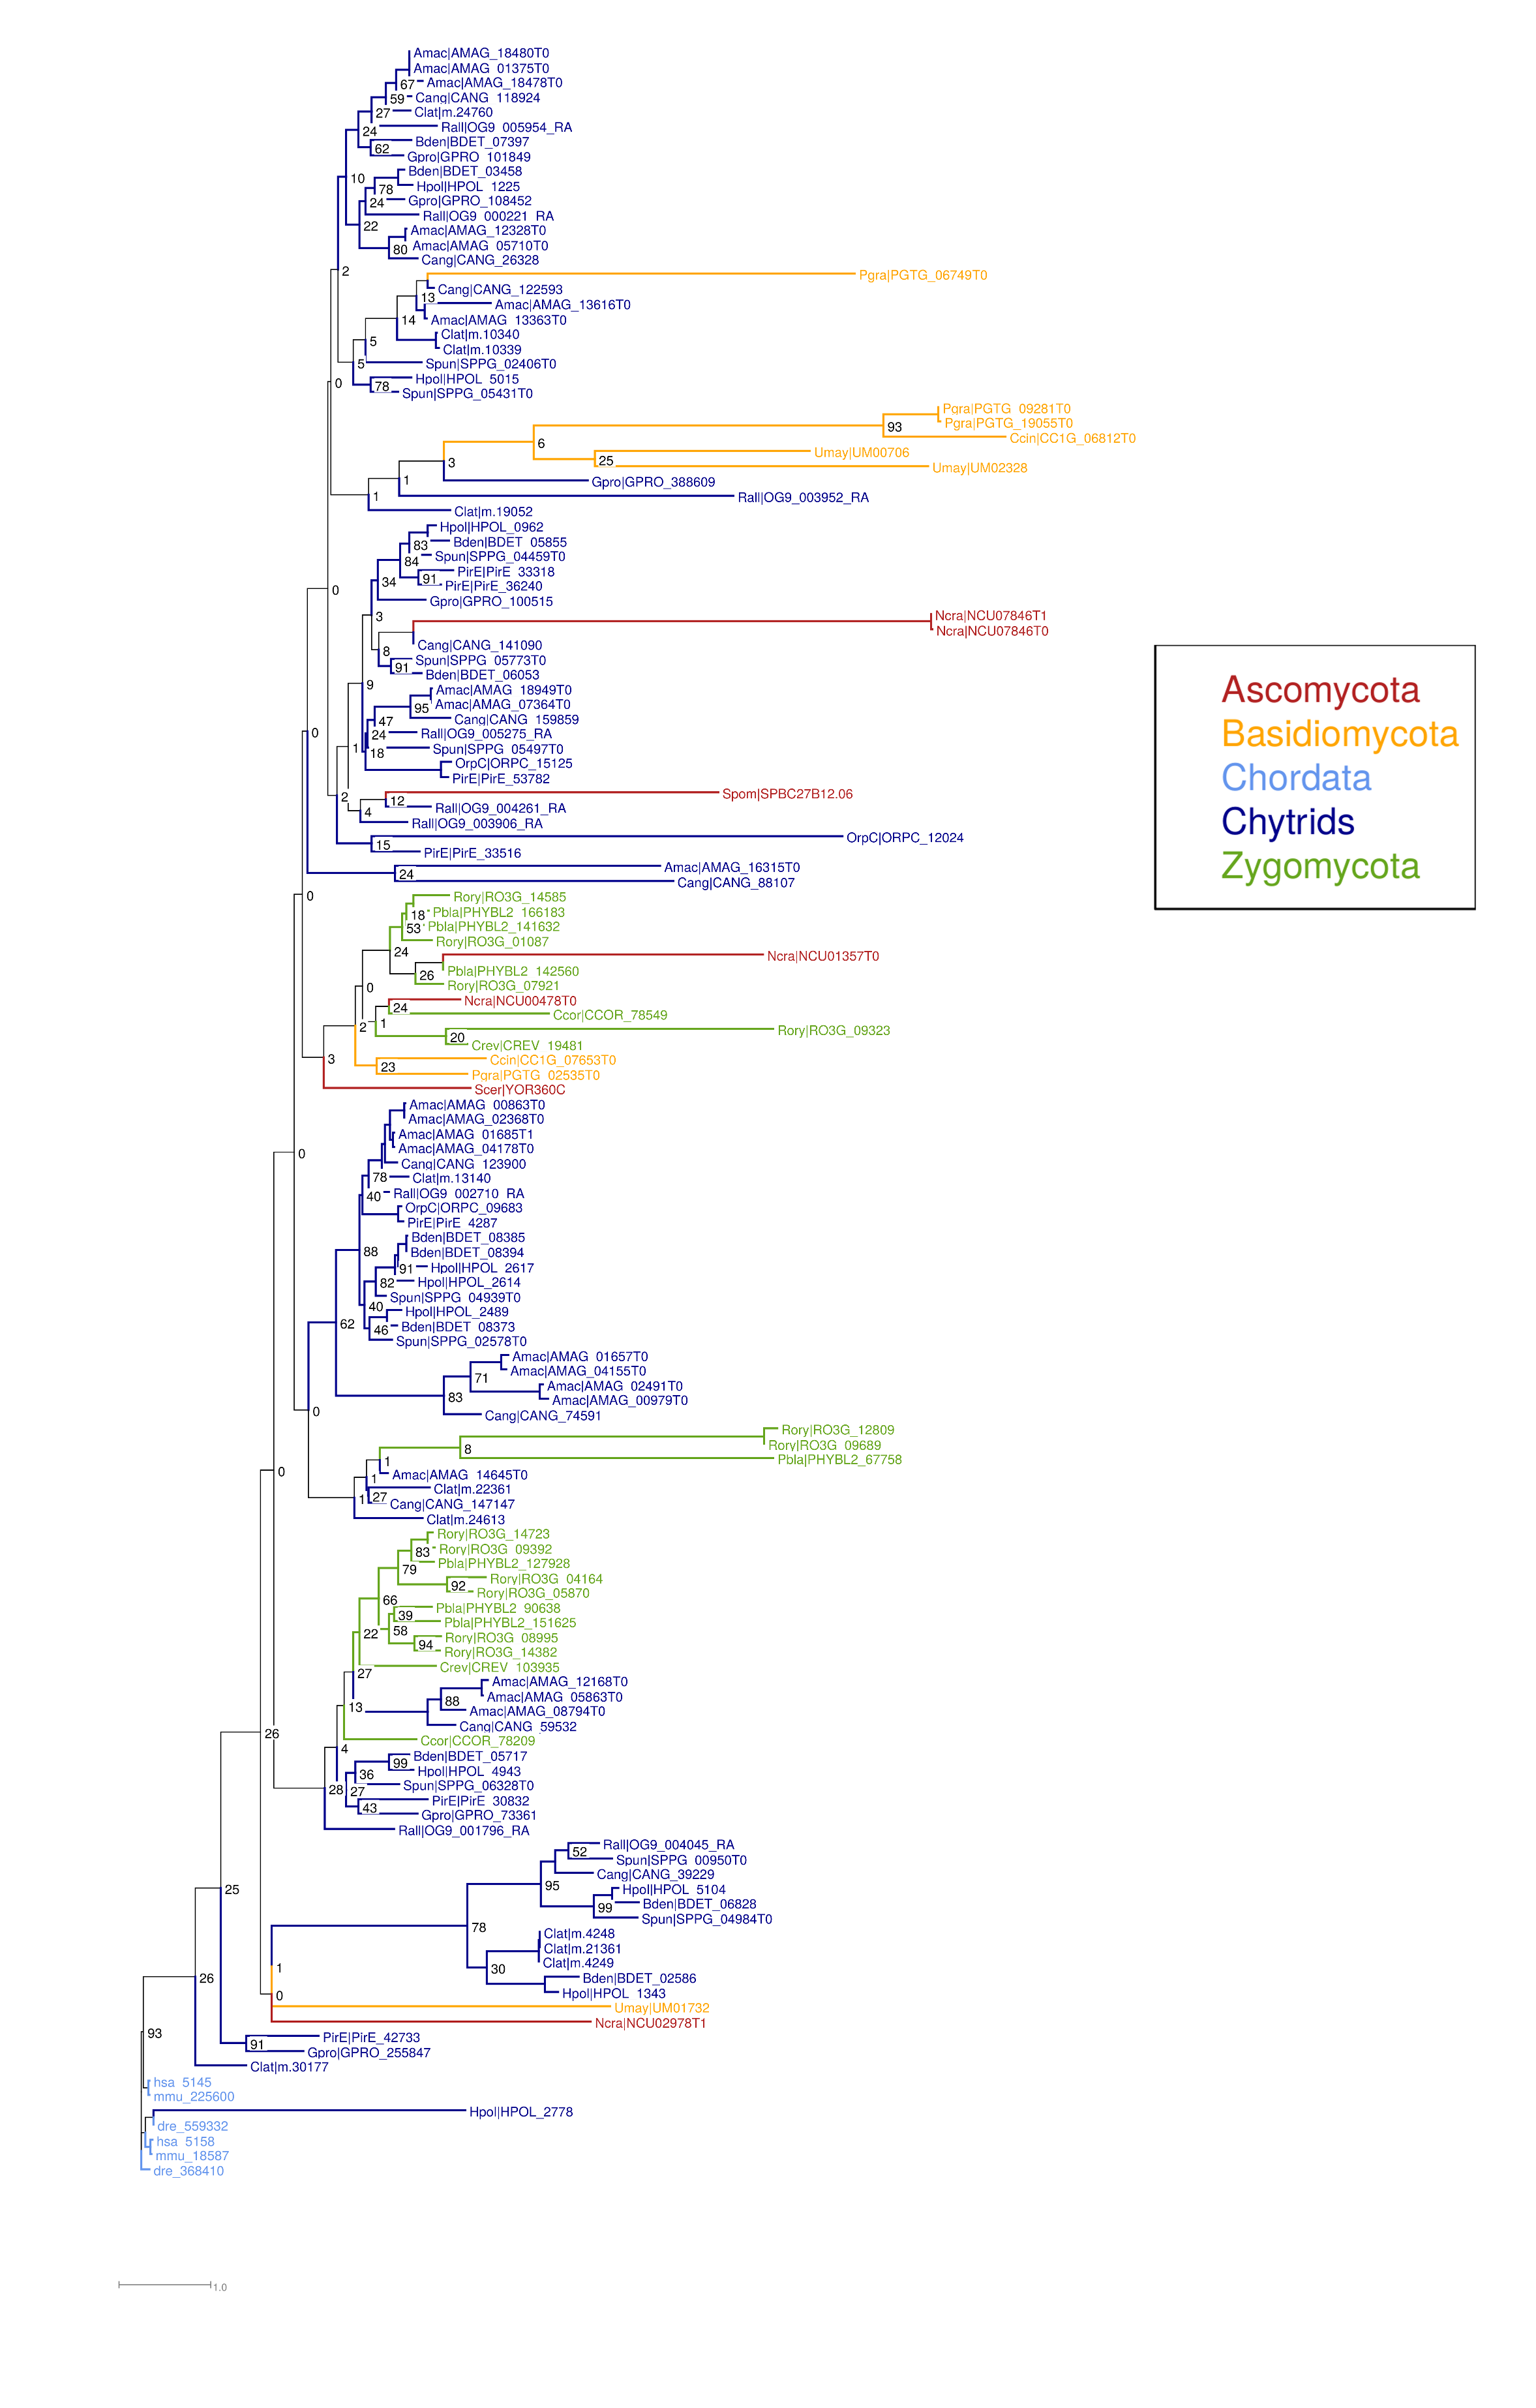
\includegraphics{./Chapter_RhodAux/img/PDE_alphaBeta_tree.png}
  \caption[PDE$\alpha$/$\beta$ tree]{Maximum likelihood tree of phosphodiesterase $\alpha$ and $\beta$ subunits recovered from HMM search in representative fungal groups. Representative metazoan sequences obtained from Uniprot are provided as outgroups.}
  \label{fig:ChRhodA_PDEtree}
\end{figure}

% Pichia gels
\begin{figure}[hb]
  \centering
  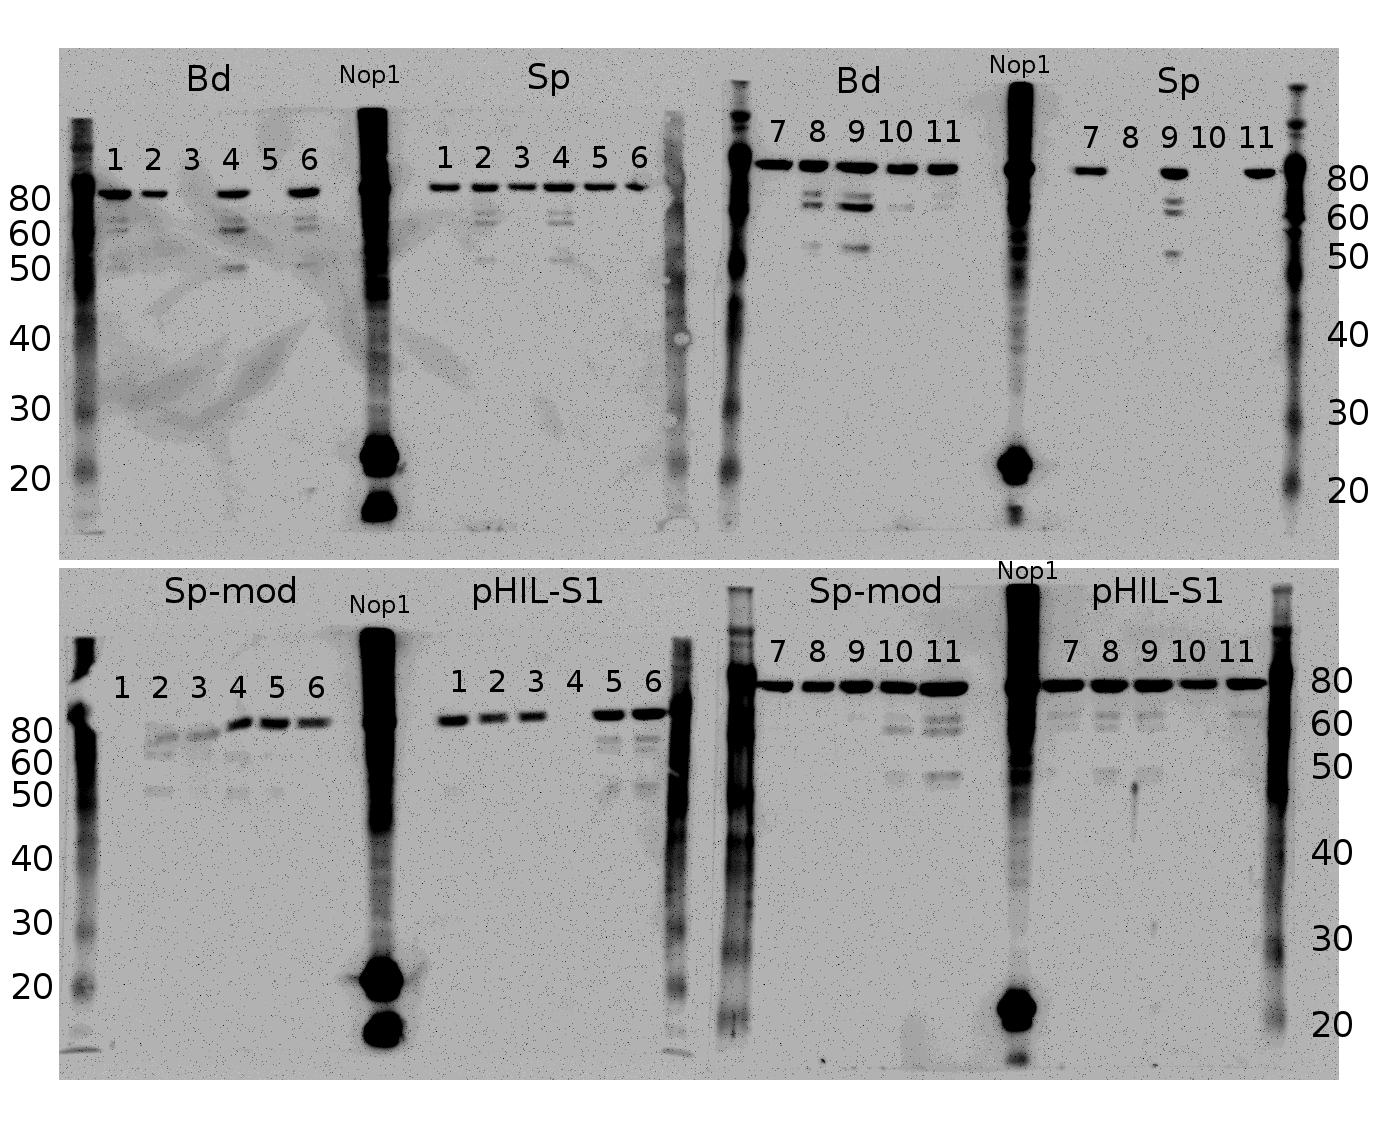
\includegraphics{./Chapter_RhodAux/img/pichia_expressionGels.png}
  \caption[\textit{P. pastoris} opsin expression]{Western blots for heterologous \textit{Pichia pastoris} expression of opsin constructs from \textit{Bd} and \textit{sp}, both native and missing lysine ("\textit{Sp}-mod"). Expression of the expected Nop-1 protein from \textit{Neurospora crassa} can be seen, and empty vector pHIL-S1 is included as a negative control.}
  \label{fig:ChRhodA_PichiaBlot}
\end{figure}
